\chapter{General Stuff}





\section{Use version control}

Use some kind of sensible version control for your code.
The author uses Git but has also heard good things about Mercurial.
Sending the code to yourself on facebook is not a proper system for version control.





\section{Use \hologo{LuaLaTeX} or \hologo{XeLaTeX}}

Use \hologo{LuaLaTeX} or \hologo{XeLaTeX} for native unicode support (i.e.\ without including any kind of additional packages).
The author recommends \hologo{LuaLaTeX} because the \texttt{microtype} package his only a limited functionality under \hologo{XeLaTeX}.





\section{Use the KOMA classes}

Instead of the standard classes \texttt{article}, \texttt{report} and \texttt{book} use the more modern KOMA-Script classes \texttt{scrartcl}, \texttt{scrreprt} and \texttt{scrbook}.
They provide more functionalities then the standard classes.
If you don’t like the standard headings style of the KOMA-Script classes then you can use the option \texttt{headings = standardclasses} to get the style of the standard classes.





\section{Split up your project in files}

Any slighty larger project should be split up into multiple files.
There are (at least) three useful ways to include another file into your project: \commandtt{usepackage}, \commandtt{include} and \commandtt{input}.
\begin{itemize}[leftmargin=*]
  \item
    Most of the preamble informations -- including of packages, configuration of syles, configuration of the look and feels of the document -- should be put into one or multiple \texttt{.sty} files.
    These file(s) can then be included into the document by using \commandtt{usepackage}.
  \item
    The commands \commandtt{include} and \commandtt{input} insert the text of the specified documents at the position where they are used, but have slight differences:
    \begin{itemize}[label = \textopenbullet, leftmargin=*]
      \item
        The \commandtt{include} command ensures that the included content starts on a new page, and also that the following content begines on a new page.
        The \commandtt{input} simply inserts the included content at the given position without any such additional formatting.
      \item
        Multiple uses of \commandtt{include} cannot be nested, i.e.\ an included file cannot contain the \commandtt{include} command again.
        The \commandtt{input} command on the other hand can be nested.
        
    \end{itemize}
\end{itemize}

One should use the \commandtt{include} command for chapters and the \commandtt{input} command for any smaller level of text organization.
One should break the main text into smaller units until the resulting files have a sensible length.

Suppose for example that your text consists of three chapters, each of which consists of two sections.
Then you should have at least ten files:
\begin{itemize}
  \item
    A master file \texttt{main.tex}.
    This file includes all other files in some way, and this is the file which needs to be compiled.
  \item
    A file \texttt{mystyle.sty} in which packages are included and options are set.
  \item
    Three files like \texttt{chapter1.tex}, \texttt{chapter2.tex} and \texttt{chapter3.tex} for the chapters.
  \item
    Sixes files for the sections, say \texttt{section1.tex} up to \texttt{section6.tex}.
\end{itemize}
These files should include each other as follows:
\begin{center}
  % the following diagram uses the "trees" library
  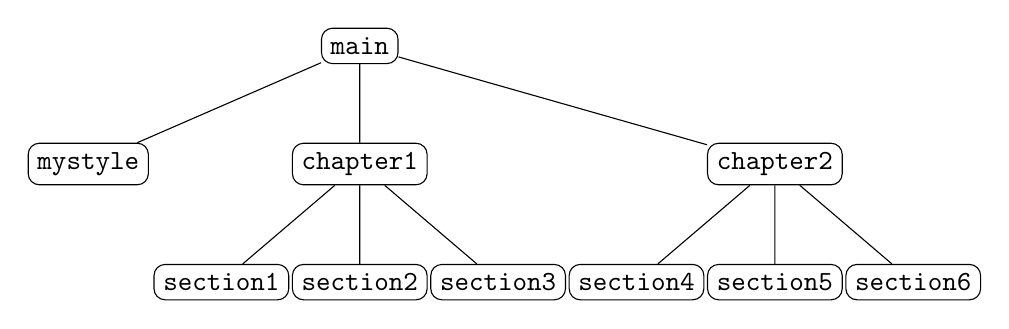
\begin{tikzpicture}[
    every node/.style = {shape=rectangle, rounded corners, draw, align=center},
    level 1/.style = {sibling distance = 15em},
    level 2/.style = {sibling distance = 5em}
    ]
    \node {\texttt{main}}
      child { node [right=3em] {\texttt{mystyle}} }
      child { node {\texttt{chapter1}}
        child { node {\texttt{section1}} }
        child { node {\texttt{section2}} }
        child { node {\texttt{section3}} }
      }
      child { node {\texttt{chapter2}}
        child { node {\texttt{section4}} }
        child { node {\texttt{section5}} }
        child { node {\texttt{section6}} }
      };
  \end{tikzpicture}
\end{center}
We suppose for simplity that all ten files are contained in the same directory.
The master file \texttt{main.tex} should look roughly as follows:
%
\begin{tcblisting}{listing only, title={\texttt{main.tex}}}
\documentclassa[a4paper, 10pt]{scrreprt}

\usepackage{mystyle}

\title{A Report}
\author{John Doe}

\begin{document}

\maketitle

\include{chapter1}
\include{chapter2}

\end{document}
\end{tcblisting}
%
The file \texttt{mystyle.sty} may look as follows:
%
\begin{tcblisting}{listing only, title={\texttt{mystyle.sty}}}
%%%%% PACKAGES

% general mathematics
\usepackage{mathtools}
\usepackage{amssymb}

% commutative diagrams
\usepackage{tikz-cd}

%%%%% NEW COMMANDS

% new operators
\DeclareMathOperator{\End}{End}
\DeclareMathOperator{\Hom}{Hom}
\end{tcblisting}
%
The file \texttt{chapter1.tex} should look roughly as follows:
%
\begin{tcblisting}{listing only, title={\texttt{chapter1.tex}}}
\chapter{Name of the first chapter}

Some introduction to this chapter before the first section appears.

\input{section1}
\input{section2}
\end{tcblisting}
%
The file \texttt{section1.tex} should look roughly as follows:
%
\begin{tcblisting}{listing only, title={\texttt{section1.tex}}}
\section{Name of the first section}

Text of the first section.
\end{tcblisting}





\section{Make use of whitespace}

\hologo{LaTeX} almost never cares about unnecessary white space in your code.
Use generous amounts of whitespace to organize your code in a sensible way.
Don’t do the following:
\begin{tcblisting}{listing only, title = {Wrong}}
\[\begin{pmatrix*}[r]a^2+b^2&a^2-b^2\\-a^2+b^2&-a^2-b^2\end{pmatrix*}\]
\end{tcblisting}
Instead do the following:
\begin{tcblisting}{listing only, title={Right}}
\[
  \begin{pmatrix*}[r]
     a^2 + b^2 &  a^2 - b^2 \\
    -a^2 + b^2 & -a^2 - b^2
  \end{pmatrix*}
\]
\end{tcblisting}
You can (and should) even do the following:
\begin{tcblisting}{listing only, title={Right}}
\[
  \begin{pmatrix*}[r]
    a^2 + b^2
    &
    a^2 - b^2
    \\
    - a^2 + b^2
    &
    - a^2 - b^2
  \end{pmatrix*}
\]
\end{tcblisting}
This last one is easiest to write and easiest to navigate.

Also put at least one space between any two symbols that do not belong together.
Don’t do the following:
\begin{tcblisting}{listing only, title={Wrong}}
$y=\sin(x)-e^x$
\end{tcblisting}
Instead do the following:
\begin{tcblisting}{listing only, title={Right}}
$y = \sin(x) - e^x$
\end{tcblisting}





\section{Write one sentence per line}

Related the previous point, write at most one sentence per line.
This has at least three advantages:
\begin{itemize}
  \item
    When an error or warning occurs \hologo{LaTeX} will (try to) tell you the line of source code in which the problem occurs.
    Having your source code split up over multiple lines makes it much easier to find the problem.
  \item
    Organizing the source code in lines will in most cases make the tools provided by your version control system (like Git) more efficient to use.
  \item
    By writing one sentence per line you will more easily spot sentences which are overly long.
\end{itemize}





\section{Properly indent your source code}

Writing \hologo{LaTeX} means writing source code.
Make sure that your source code is properly indented.





\section{Don’t ignore warnings}

There are two ways in which \hologo{LaTeX} will tell you that something went wrong:
Errors and warnings.

The occurence of an error means that \hologo{LaTeX} was unable the process the source code and gave up at some point in the process.
In the case of a warning \hologo{LaTeX} again wasn’t able to process the source code, but decided to produce some output nevertheless.
Hence the only difference between an error and a warning is how \hologo{LaTeX} decided to proceed with it.
But there is no intrinsic difference between the two of them.

It is typically hard to ignore errors, as no output file will be generated.
But warnings also shouldn’t be ignored:
While the occurance of an error means that you get no outupt at all, the occurance of a warning means that you’re getting a faulty output.

% TODO: Too many warnings make future problems worse.
